\documentclass{beamer}

\usepackage{pgfpages}
% \setbeameroption{show notes on second screen}


% Note rendering settings
% \setbeameroption{hide notes} % Default
% \setbeameroption{show notes}
% \setbeameroption{show only notes}

% % \textcolor
\usepackage{xcolor}

% Maths
\usepackage{mathabx}
\usepackage{mathtools}

% Algorithms using algorithmicx package (with its algpseudocode command set)
\usepackage{algpseudocode}

% Operators for common operations
\DeclareMathOperator{\DFT}{DFT}
\DeclareMathOperator{\FFT}{FFT}

% Code listings
\usepackage{listings}
\usepackage{lstautogobble}
\lstset{
		basicstyle=\small,
		breaklines=true,
		autogobble=true,
		postbreak=\mbox{$\drsh$},
}

% Date management
\usepackage{datetime2}
\DTMsavedate{presentation}{2021-12-14}

% BibLaTeX
\usepackage[
  style=alphabetic,
  backend=biber, % Default backend, just listed for completness
  sorting=ynt % Sort by year, name, title
]{biblatex}
\addbibresource{references.bib}
\nocite{*}

% User numeric labels (instead of icons) in bibliography page
\setbeamertemplate{bibliography item}{\insertbiblabel}

% Somber theme with right-justified headings
\usetheme{Pittsburgh}

% Red colour for headings
% \usecolortheme{beaver}

% Rectangles (instead of ugly dots) for enumeration bullet points
\useinnertheme{rectangles}

% Gray (instead of the default blue) for bullet points
% \setbeamercolor{itemize item}{fg=gray}
% \setbeamercolor{itemize subitem}{fg=gray}

\title{Schönhage–Strassen Algorithm for Fast Multiplication}

\author{Michael Senn}
\institute{Faculty of Science, University of Bern}
\date{\DTMusedate{presentation}}

\begin{document}
\begin{frame}
		\titlepage

		\note[item]{Welcome to my presentation for this seminar, we'll be talking about ...}
\end{frame}

% Only show sections
\setcounter{tocdepth}{1}
\begin{frame}
		\frametitle{Outline}
		\frametitle{\secname}
		\framesubtitle{\subsecname}
		\tableofcontents
		\note{Will introduce the problem, and outline some earlier methods}
		\note{Briefly explain mathematical concepts of DFT and convolution theory}
		\note{Moving on to using the FFT for fast multiplication}
		\note{Culminating in the Schönhage-Strassen algorithm}
\end{frame}

\section{Introduction}

\begin{frame}
		\frametitle{\secname}

		\textbf{Goal: Multiplying large integers}

		\begin{itemize}
				\item Given $x, y$ two $n$-bit integers
				\item Where $x = x_0, x_1, \ldots, x_{n-1}$, $y = y_0, y_1, \ldots, y_{n-1}$ big-endian representation
				\item Calculate $z \coloneqq x \cdot y$
		\end{itemize}
\end{frame}

\subsection{Long multiplication}

\begin{frame}
		\frametitle{\secname}
		\framesubtitle{\subsecname}

		\begin{itemize}
				\item Multiply digit by digit, sum up the products
				\item Complexity: $O(n^2)$ additions and multiplications
				\item Up to 1960: Long multiplication conjectured to be asymptotically optimal
				\item We can do better
		\end{itemize}
\end{frame}

\subsection{Karatsuba algorithm}

\begin{frame}
		\frametitle{\secname}
		\framesubtitle{\subsecname}

		\begin{itemize}
				\item Anatoly Karatsuba, 1960
				\item Idea: Work in large base $W$
				\item $x = x_0 + x_1 \cdot W$, where $x_0, x_1 \in [0, W - 1]$
				\item Karatsuba relation
						\begin{align*}
								xy & = \frac{t + u}{2} - v + \frac{t - u}{2} \cdot W + v \cdot W^2 \\ 
								t & = (x_0 + x_1) \cdot (y_0 + y_1) \\
								u & = (x_0 - x_1) \cdot (y_0 - y_1) \\
								v & = x_1 \cdot y_1
						\end{align*}
				\item Replaces one multiplication of two $2n$-digit numbers
						with three multiplications of $n$-digit numbers
				\item Divide and conquer: Asymptotic complexity of
						$O(n^{\log_2{3}}) \approx O(n^{1.58})$
		\end{itemize}
\end{frame}

\subsection{Toom-Cook method}

\begin{frame}
		\frametitle{\secname}
		\framesubtitle{\subsecname}

		\begin{itemize}
				\item Toom 1963, Cook 1966
				\item Idea: Interpret digits of $x$ and $y$ as coefficients of polynomial of degree $D - 1$
				\item $x(t) = x_0 + x_1 \cdot t + \ldots + x_{D-1} \cdot t^{D-1}$
				\item $z(t) \coloneqq x(t) \cdot y(t)$ has degree $2D - 2$
				\item Evaluate $z(t)$ at $2D - 1$ values
				\item Reconstruct coefficients of polynomial $z(t)$
				\item For $D = 3$, asymptotic complexity of $\approx O(n^{1.46})$
		\end{itemize}
\end{frame}

\section{Discrete Fourier Transform (DFT)}

\begin{frame}
		\frametitle{\secname}

		\textbf{Goal}: Perform Fourier analysis of discrete signal $x = (x_0,
		x_1, \ldots, x_{n-1})$ in some algebraic field.
		\note{Usual definition over field of complex numbers. We will (later) use it over a finite field}

		\begin{align*}
				\operatorname{DFT}(x): X_i & = \sum_{i=0}^{n-1} x_i \cdot g^{-i \cdot k} \\
				\operatorname{DFT}^{-1}(X): x_i & = \frac{1}{n} \sum_{i=0}^{n-1} X_i \cdot g^{i \cdot k}
		\end{align*}

		Where $g$ is a primitive $n$-th root of unity (i.e. $g^n = 1$, $g^m
		\neq 1 \forall m < n$)
\end{frame}

\subsection{Calculating the DFT}

\begin{frame}
		\frametitle{\secname}
		\framesubtitle{\subsecname}

		\begin{itemize}
				\item Naive approach would be $O(n^2)$
				\item Recall first presentation: FFT algorithm allows calculation in $O(n \log(n))$
				\item We'll use FFT as blackbox: $\FFT(x) = \DFT(x)$.
		\end{itemize}
\end{frame}

\section{Convolution theory}

\begin{frame}
		\frametitle{\secname}

		Given two signals $f$ and $g$, their convolution is defined as:
		\[
				(f * g)(t) \coloneqq \int_{-\infty}^{\infty} f(\tau) \cdot g(t - \tau) d\tau
		\]

		\note{Applications in signal \& image processing, computer vision, pure mathematics, ...}
		
		\textbf{However} we work with finite signals. We introduce four types
		of discrete convolution operations. Consider finite signals $x, y$
\end{frame}

\subsection{Cyclic convolution}

\begin{frame}
		\frametitle{\secname}
		\framesubtitle{\subsecname}

 		\begin{columns}
 				\column{0.5\textwidth}
				\textbf{Cyclic} convolution $z = x \times y$ is $n$-length discrete
				signal with components:
				\[
						z_k \coloneqq \sum_{i + j \equiv k \pmod{n}} x_i \cdot y_j
				\]
				\note{Symmetry is result of commutativity in field}
 				\column{0.5\textwidth}
 				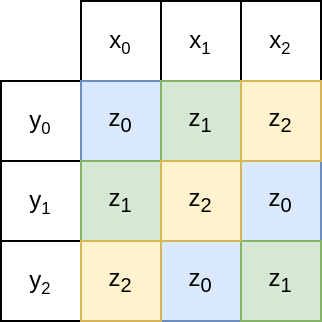
\includegraphics[width=\textwidth]{../resources/cyclic_convolution.drawio.png}
		\end{columns}
\end{frame}

\subsection{Acyclic convolution}

\begin{frame}
		\frametitle{\secname}
		\framesubtitle{\subsecname}

 		\begin{columns}
 				\column{0.5\textwidth}
				\textbf{Acyclic} convolution $u = x \times_A y$ is $2n$-length discrete
				signal with components:
				\note{Observe: Acyclic separates cylic into those where addition `wrapped around' vs those where it didn't}
				\begin{align*}
						u_k & \coloneqq \sum_{i + j = n} x_i \cdot y_j \\
						u_{2n - 1} & \coloneqq 0
				\end{align*}
 				\column{0.5\textwidth}
 				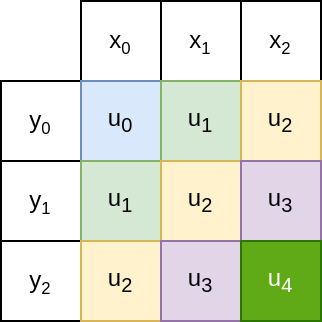
\includegraphics[width=\textwidth]{../resources/acyclic_convolution.drawio.png}
		\end{columns}
\end{frame}

\subsection{Negacyclic convolution}

\begin{frame}
		\frametitle{\secname}
		\framesubtitle{\subsecname}

 		\begin{columns}
 				\column{0.5\textwidth}
				\textbf{Negacyclic} convolution $v = x \times_\_ y$ is $n$-length discrete
				signal with components:
				\[
						v_k \coloneqq \sum_{i + j = n} x_i \cdot y_j - \sum_{i + j = n + k} x_i \cdot y_j
				\]
 				\column{0.5\textwidth}
 				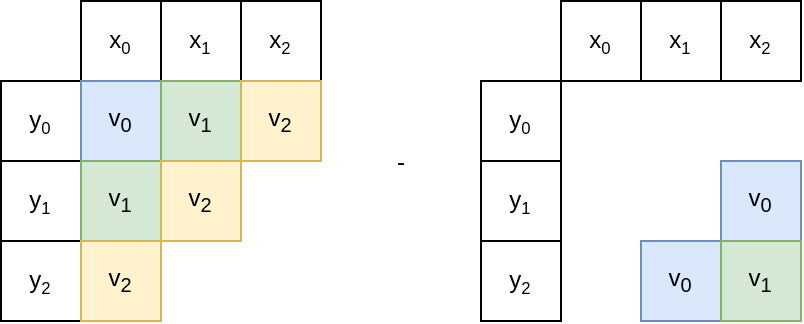
\includegraphics[width=\textwidth]{../resources/negacyclic_convolution.drawio.png}
		\end{columns}
\end{frame}

\subsection{Half-cyclic convolution}

\begin{frame}
		\frametitle{\secname}
		\framesubtitle{\subsecname}

 		\begin{columns}
 				\column{0.5\textwidth}
				\textbf{Half-cyclic} convolution $w = x \times_H y$ is $n$-length discrete
				signal with first $n$ components of acyclic convolution $x \times_A y$:
				\[
						w_k \coloneqq (x \times_A y)(k)
				\]
 				\column{0.5\textwidth}
 				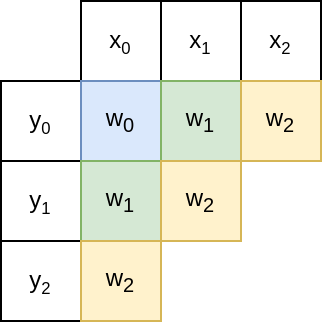
\includegraphics[width=\textwidth]{../resources/halfcyclic_convolution.drawio.png}
		\end{columns}
\end{frame}

\subsection{Relation between convolutions}

\begin{frame}
		\frametitle{\secname}
		\framesubtitle{\subsecname}

		Convolutions are related. Being able to e.g. calculate cyclic and
		negacyclic allows to also calculate half-cyclic or acyclic
		convolutions.

		\begin{align*}
				x \times_H y & = \frac{1}{2} \cdot ((x \times y) + (x \times_{\_} y)) \\
				x \times_A y & = (x \times_H y) || \frac{1}{2} \cdot ((x \times y) - (x \times_{\_} y)) \\
				L(x) \times_A L(y) & = x \times y = x \times_{\_} y\text{, where } n = 2k, x_i = y_i = 0 \forall i \geq k
		\end{align*}
		\note{$L$ here is left half of signal of length $2n$}
\end{frame}

\subsection{Convolution theorem}

\begin{frame}
		\frametitle{\secname}
		\framesubtitle{\subsecname}

		\note{Now we want to tie together convolutions and DFT}

		We can calculate the cyclic convolution using the DFT:
		\[
				x \times y = \DFT^{-1}(\DFT(x) \cdot \DFT(y))
		\]

		\note{The multiplication here is component-wise multiplication}

		This is $O(n \log n)$ instead of the naive $O(n^2)$ if using the FFT.
\end{frame}

\subsection{Multiplication is a type of convolution!}

\begin{frame}
		\frametitle{\secname}
		\framesubtitle{\subsecname}

		\note{Why do we care about convolutions?}

		Consider long multiplication with a delayed carry operation.
		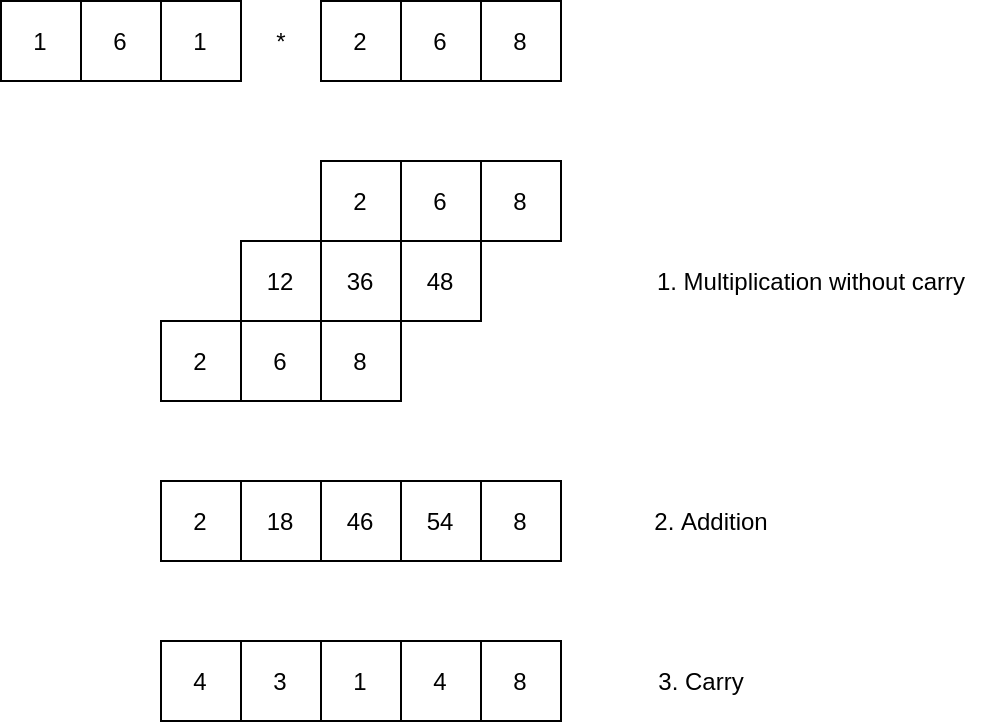
\includegraphics[width=0.7\textwidth]{../resources/long_multiplication.drawio.png}
\end{frame}

\begin{frame}
		\frametitle{\secname}
		\framesubtitle{\subsecname}

		The multiplication part is an acyclic convolution.
		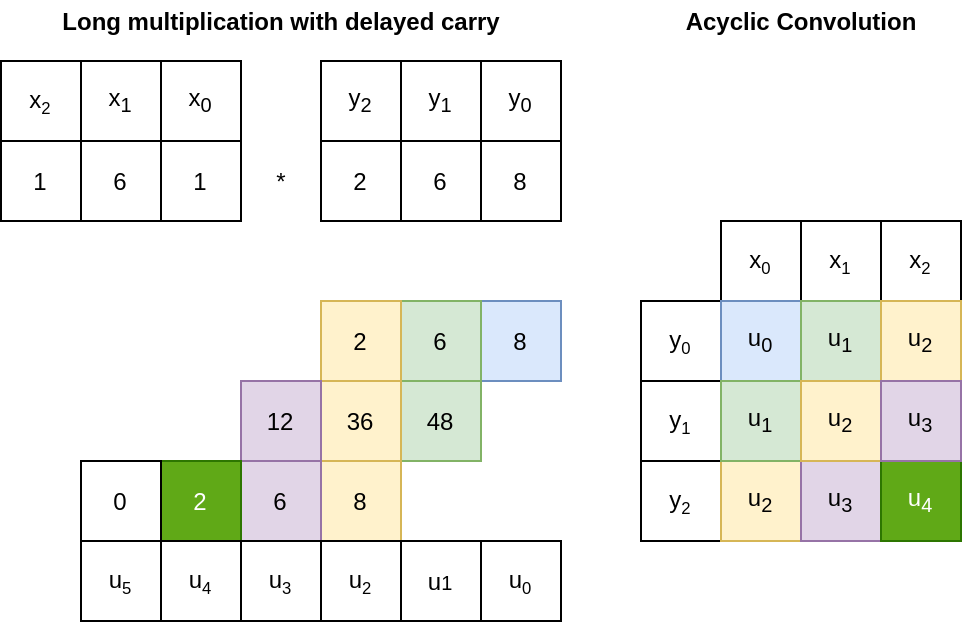
\includegraphics[width=0.7\textwidth]{../resources/multiplication_convolution.drawio.png}
\end{frame}

\section{FFT Multiplication}

\begin{frame}
		\frametitle{\secname}

		Given $x, y$ two $n$-digit integers in base $B$, start by zero-padding.

		\begin{algorithmic}[1]
				\Function{FFTMult}{$x, y$} \Comment{$x, y$ $n$-digit base-$B$ integers}
				\State $x \gets$ \Call{Pad}{x, 2n} \Comment{Zero-pad to length $2n$ on right side}
				\State $y \gets$ \Call{Pad}{y, 2n}
				\algstore{fftmult}
		\end{algorithmic}
\end{frame}

\begin{frame}
		\frametitle{\secname}

		Calculate the acyclic convolution $x \times_A y$ by means of the
		convolution theorem. Mind that we must round the results, as we might
		be in an arbitrary field such as the field of complex numbers!

		\begin{algorithmic}[1]
				\algrestore{fftmult}
				\State $X \gets$ \Call{DFT}{x}
				\State $Y \gets$ \Call{DFT}{y}
				\\
				\State $Z \gets X \times Y$ \Comment{Dyadic product}
				\\
				\State $z \gets$ $\Call{DFT}{Z}^{-1}$
				\State $z \gets$ \Call{round}{z}
				\algstore{fftmult}
		\end{algorithmic}
\end{frame}

\begin{frame}
		\frametitle{\secname}

		Finally perform the carry operation and return the result.

		\begin{algorithmic}[1]
				\algrestore{fftmult}
				\State $carry \gets 0$
				\For{$i \gets 0$ to $2n$}
				  \State $v \gets z_i + carry$
				  \State $z_n \gets v \mod B$
				  \State $carry \gets v / B$ \Comment{Integer division}
				\EndFor
				\State \textbf{Return} $carry || z_n || \ldots || z_0$ \Comment{Optionally remove leading 0s}
				\EndFunction
		\end{algorithmic}
\end{frame}

\section{Schönhage-Strassen algorithm}

\section{Summary}

\begin{frame}
		\frametitle{References}
		\printbibliography
\end{frame}

\end{document}
